
\begin{figure*}
  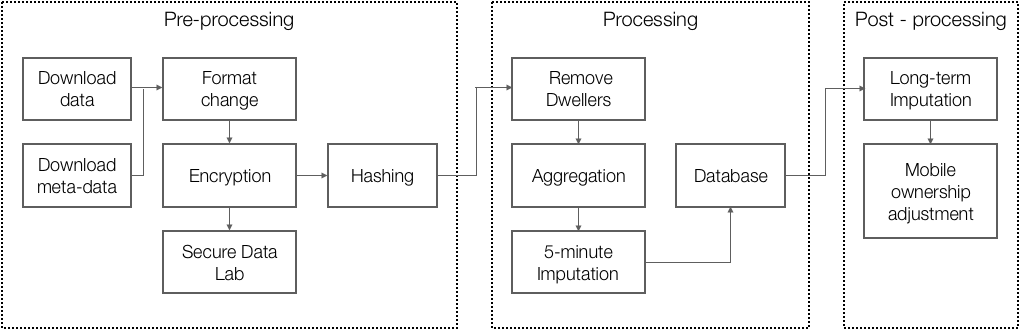
\includegraphics[trim={0 0 0 0},clip]{images/processing-pipeline-full.png}
  \caption{The complete data processing pipeline which takes in raw probe requests from Smart Street Sensor project and outputs footfall estimations.}
  \label{figure:processing:pipeline:full}
\end{figure*}

%==============================================================================%
\section{Data pipeline} \label{section:pipeline}
%==============================================================================%

After the discussion of the toolkit and the methods, the final step of this research was to convert the Wi-Fi probe requests to footfall. 
This meant devising a processing pipeline which combines the `data toolkit' and the methods together, takes the probe requests generated by the Smart Street Sensor as input and generates a best possible estimation of footfall estimations as output. 
Figure \ref{figure:processing:pipeline:full} illustrates the pipeline that was devised as part of this research.
The code which implements this pipeline is detailed in Appendix \ref{appendix:data:pipeline}.
The pipeline comprises of three parts,
\begin{itemize}
  \itemsep-0.25em
  \item \textit{Pre-processing} - where the data gets transformed and modified for security and convenience.
  \item \textit{Processing} - where the data gets converted to estimated ambient population.
  \item \textit{Post-processing} where the general population estimate gets adjusted to better reflect information that was sought - footfall in this case.
\end{itemize}

%------------------------------------------------------------------------------%
\subsection{Pre-processing}
%------------------------------------------------------------------------------%
The aim of \textit{pre-processing} was primarily to convert the dataset comprising of probe requests into a form which can be processed quickly and conveniently.
In the case of the Smart Street Sensor project, the data is retrieved from the \textit{Azure} store and converted from JSON format into CSV file for each location on a given day.
These files were stored in directories within a file system hierarchy of year, month and date providing us an efficient storage system as discussed in Section \ref{section:toolkit}.

The secondary aim of pre-processing was to anonymise the data using cryptographic hashing and encryption to protect the privacy of the users.
The MAC address field in the dataset was converted into an unique hash value using SHA256 algorithm to avoid linking this dataset with other sources of MAC address data and a random salt value was introduced every week to avoid timing attacks where sufficiently long term information on hashes could be de-anonymised by correlating the precise time they occur in other datasets.
Although this is not theoretically fool-proof, this made sure that dataset could not used to personally identify the users within practical means.
Finally, the non-hashed raw data were encrypted using RSA algorithm and physically transferred to an isolated secure facility for storage.
Thus preserving the unmodified information for further investigation, if required.

%------------------------------------------------------------------------------%
\subsection{Processing}
%------------------------------------------------------------------------------%
The processing of the data involved the implementation of the methods discussed in Section \ref{section:processing}.
First the probe requests were separated into global and local based on the OUI present in them. 
The non-randomised, global probe requests were then aggregated into ambient population estimation employing the following steps,

\begin{enumerate}
  \item Signal strength filtering - as discussed in section \ref{section:processing} the probe requests with signal strengths less than the \textit{threshold} (Calculated dynamically from the previous 24 hour period) were filtered out.t
  \item Removal of dwellers - The probes with MAC addresses which are repeated within the past 30 minutes were removed to eliminate noise caused by devices which are dwelling around the sensor for a long time.
  \item Aggregation - The remaining probe requests were aggregated by their MAC addresses to arrive at the count of unique MAC addresses at every five minute interval.
\end{enumerate}

The above process results in the number of devices that were present around the sensor which did not randomise their MAC addresses. 
The ratio between this `count' and the original number of probes requests with global MAC addresses gives us the \textit{compression factor} as discussed in Section \ref{section:processing}.
This factor was calculated for every interval and in turn used to calculate the number of devices which randomise their MAC addresses.
The sum of the both counts gives us the estimate of ambient population at the locations for five minute intervals.
As the final step, the gaps in the data which are shorter than fifteen minutes are filled in by imputation based on \textit{Kalman smoothing} resulting a more continuous dataset.

%------------------------------------------------------------------------------%
\subsection{Post-processing}
%------------------------------------------------------------------------------%
The post-processing involved adjusting the estimated ambient population further to match it to the real footfall counts as closely as possible.
The primary steps involved were, adjusting using manual counts, imputing missing data and adjusting for increase in mobile device ownership.
The manual adjustment was done through a global adjustment factor which is calculated for each location by comparing the footfall measured with the sensor to the footfall counted at the corresponding locations manually.
The manual counting were done for short intervals ranging from 15-30 minutes immediately after the installation of the sensors and are refreshed for selected locations yearly.
This adjustment factor, which could be greater or less than 1, was then applied on sensor counts to account for over- and under-counting at these locations.
This adjustment removes the noise caused by the location specific configuration.
In addition to this the counts since the beginning of the project were offset by 0.2\% per week to account for the increasing mobile phone ownership over the years in the United Kingdom\cite{deloitte2018}.
Finally, long term gaps in term of hours, days and weeks were filled using a seasonally decomposed method hierarchically where the daily and weekly periodicity of the counts were taken into account during the imputation process.
This ensured the final counts produced from the processing are continuous and standard enough for carrying out further research using them.
